\chapter{Frontier orbitals and partial charges}
\label{ch:density-views}
\eccexample{Examples > Getting Started}
\helppage{natural-population-analysis}
\label{sec:dv-fmo}
\index{Frontier orbitals}\index{Molecular orbitals}\index{HOMO}\index{LUMO}\index{Diels--Alder reaction}\index{Natural population analysis}\index{Hirshfeld charges}
\index{Butadiene!frontier orbitals}\index{Ethene!frontier orbitals}

Before we calculate a reaction, it is worth asking what brings the two molecules together. For the Diels--Alder reaction of butadiene with ethene there are two candidates: the attraction between partial charges on the atoms that form the new bonds, and the overlap between the highest occupied orbital (HOMO) of one molecule and the lowest unoccupied orbital (LUMO) of the other. In this chapter we look at both for the two reactants, using the gauche butadiene and the ethene optimised in Chapter~\ref{ch:scans}. The reaction itself is the subject of Chapter~\ref{ch:reaction-rates}.

\section*{This requires}
\index{Requirements!ORCA}
ORCA, as in Chapter~\ref{ch:scans}. The natural charges are computed by ECCE itself from the stored orbitals, so no NBO program is needed.

\section{Background}
\index{Partial charges!models}
A partial charge is not something a molecule has in the way it has a dipole moment; it is the result of a rule for dividing the electron density among the atoms, and different rules give different numbers. Natural population analysis (NPA) assigns the density to natural atomic orbitals, which makes its charges stable when the basis set changes. Hirshfeld charges divide the density at each point in proportion to the densities of the free atoms, which gives much smaller charges. We should therefore compare charges only within one scheme, and look for signs and trends rather than for the values themselves.

In frontier orbital theory, the [4+2] cycloaddition is allowed because the HOMO of one partner and the LUMO of the other have the same symmetry with respect to the mirror plane that both keep along the reaction, so that their lobes at the two reacting ends can overlap in phase at once. The smaller the energy gap between the two orbitals, the stronger the interaction. Note that the energies of Kohn--Sham orbitals from a DFT calculation are not ionisation or attachment energies, so we compare them only with each other, from the same method.

\section{What ECCE shows}
\index{MOs panel}
For any calculation that stores orbitals, the \menu{MOs} panel lists every orbital with its energy, occupation, symmetry and composition by atom and shell, and draws the selected one as a surface. Under \menu{Properties > Charges} are the charge schemes the code wrote, and Natural (NPA) charges that ECCE computes itself from the stored orbitals, the same way for every code; \cmd{ecce-npa} gives them on the command line. The \menu{Density Map}, \menu{Density Profile} and \menu{Surfaces} panels show the density and the orbitals in a plane, along a line and in three dimensions.

\section{Procedure}
\index{MOs panel}\index{Charges!Natural (NPA), computed by ECCE}
\begin{enumerate}
	\item Open the finished gauche-butadiene calculation of Chapter~\ref{ch:scans} in the Viewer (\menu{Tools > Viewer...}) and choose \menu{Properties > Orbitals > MOs}. The table lists every orbital with its energy, occupation, symmetry and the atoms it sits on; the HOMO is selected when the panel opens.
	\item Click \ctrl{Compute} to draw the selected orbital as a surface, then select the next row, the LUMO, and click \ctrl{Compute} again. The line below the table gives each orbital's composition by atom and shell.
	\item Choose \menu{Properties > Charges > Natural (NPA) Charges, computed by ECCE}. The charges are calculated when the row is first selected and are kept with the calculation; tick \ctrl{Show in viewer} to colour the atoms by charge. Choose \menu{Hirshfeld Charges} for comparison.
	\item Repeat the three steps for the ethene calculation.
\end{enumerate}
The same natural charges are printed on the command line by \cmd{ecce-npa}, with the populations of each shell and the natural electron configuration of each atom.

\section{Results}
\index{Butadiene!charges}\index{Ethene!charges}
Table~\ref{tab:dv-charges} gives the charges of the carbon atoms. In both schemes the terminal carbons of butadiene, C1 and C4, and the carbons of ethene are negative, and they are the atoms that form the two new bonds. Since like charges repel, the partial charges cannot be what draws the reacting carbons together. The two schemes differ by a factor of five in the size of the charges, which is the point made above: only the sign and the order are worth comparing.

\begin{table}[htbp]
	\centering
	\caption{Partial charges (in $e$) of the carbon atoms of gauche butadiene and ethene, B3LYP-D3BJ/def2-TZVP.}
	\label{tab:dv-charges}
	\begin{tabular}{lrr}
		\hline
		Atom & NPA & Hirshfeld \\
		\hline
		Butadiene C1, C4 (terminal) & $-0.365$ & $-0.071$ \\
		Butadiene C2, C3 (central) & $-0.220$ & $-0.030$ \\
		Ethene C & $-0.379$ & $-0.068$ \\
		\hline
	\end{tabular}
\end{table}

The frontier orbitals tell a different story (figure~\ref{fig:dv-homo-lumo}). The HOMO of butadiene, at $-6.59$~eV, is the $\pi$ orbital usually called $\psi_2$: the MOs panel puts 32\,\% of it on each of C1 and C4 and 16\,\% on each of C2 and C3, with a node across the central bond. Its lobes at the two ends have opposite sign above the molecular plane, which is the same pattern as in the $\pi^*$ LUMO of ethene, at $-0.05$~eV, so the two overlap in phase at both new bonds. The LUMO of butadiene ($\psi_3$, $-1.02$~eV) and the HOMO of ethene ($\pi$, $-7.57$~eV) match in the same way.

\begin{figure}[htbp]
	\centering
	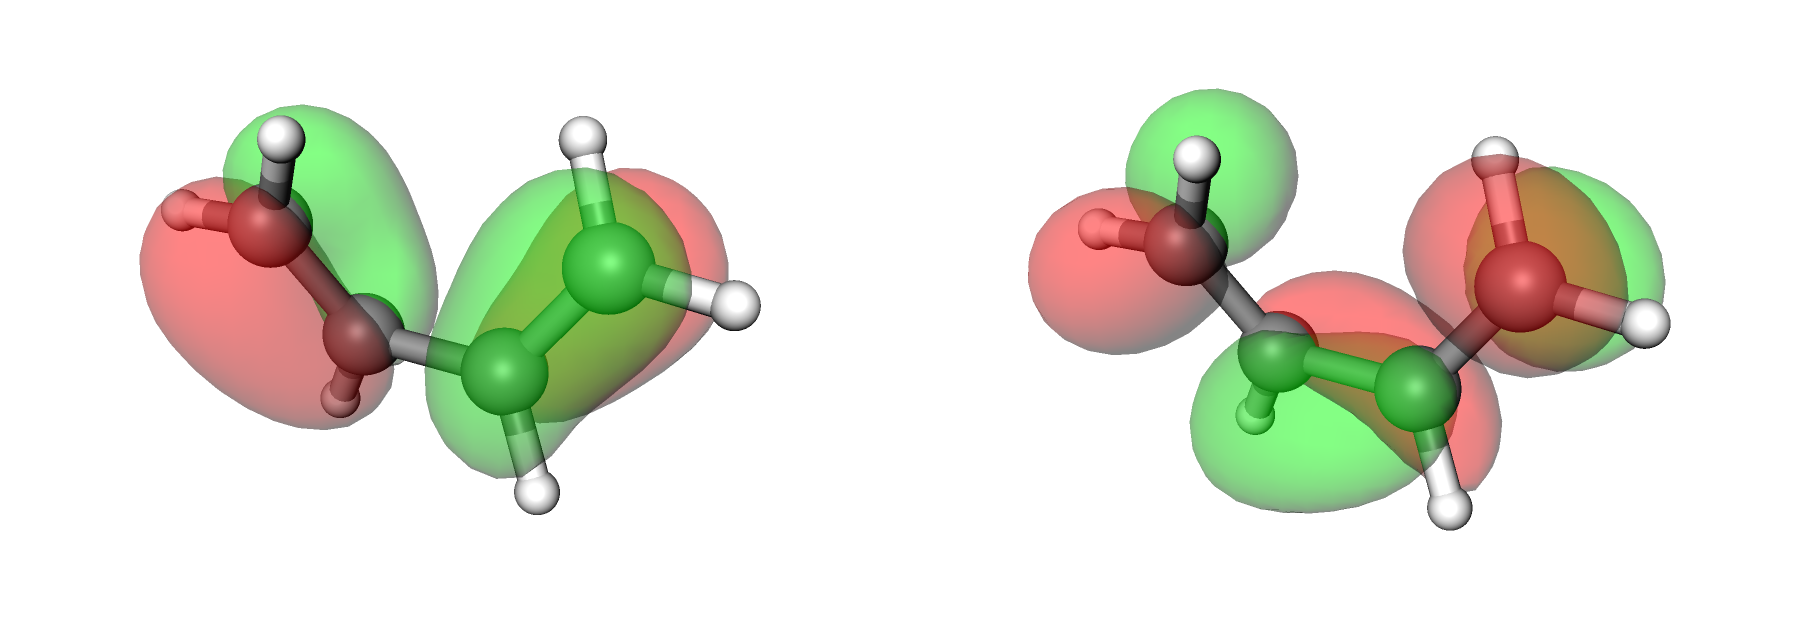
\includegraphics[width=0.9\linewidth]{density-views/homo-lumo-scis.ecce-9.5.3-dev.png}
	\caption{The HOMO (left, $\psi_2$) and the LUMO (right, $\psi_3$) of gauche butadiene, computed in the \menu{MOs} panel and seen from the same direction, onto the carbon chain with the molecule tilted about \ang{25} from face-on; the two colours are the two signs of the orbital. In the HOMO each half of the molecule, a terminal and a central carbon, carries one lobe of the same sign, and the sign changes across the central C2--C3 bond: there is a node between C2 and C3. In the LUMO the sign changes across each terminal bond, C1--C2 and C3--C4, and the two central carbons share one lobe across C2--C3.}
	\label{fig:dv-homo-lumo}
\end{figure}

The two possible gaps are almost the same: \SI{6.54}{eV} from the HOMO of butadiene to the LUMO of ethene, and \SI{6.55}{eV} from the HOMO of ethene to the LUMO of butadiene. For the parent reaction, neither direction of electron flow is preferred, and both interactions together make the reaction go. Substituents change this: an electron-donating group on the diene raises its HOMO and an electron-withdrawing group on the dienophile lowers its LUMO, which narrows the first gap and is why such pairs react much faster. So the answer to the question we started with is that the reaction is controlled by orbital overlap, not by the charges.

\XXX[figure: ethene HOMO and LUMO seen from the side (retake once ECCE lights a turned view from the camera); figure: NPA charges on the atoms]

\section{Coupling with other codes}
% What feeds this calculation (a cheaper screen, a structure from another code)
% and what it feeds (refinement, a property from the code best at it); which
% hand-off is made (usually by hand: a new calculation from this one's
% structure or orbitals in another code); a workflow only where it pays.
Natural charges computed by ECCE come from the orbitals that ECCE stores for every code, so a charge from an ORCA calculation and one from a Gaussian or ECCE-QM calculation are defined the same way, and a structure handed from one code to another keeps a comparable set of charges.
